\documentclass[12pt]{article}
\usepackage{amsmath}
\usepackage{amsthm}
\usepackage[english]{babel}
\usepackage{float}
\usepackage{graphicx}
\usepackage{amssymb}
\usepackage{hyperref}
\usepackage[utf8]{inputenc}
\usepackage{listings}
\usepackage{pgf, tikz}
\usepackage{xcolor}
\usepackage{geometry}
\geometry{margin=1in}
\usepackage[utf8]{inputenc}
\newtheorem{theorem}{Theorem}
\newtheorem{example}{Example}
\newtheorem{remark}{Remark}[section]
\newtheorem{definition}{Definition}[section]
\theoremstyle{definition}
% Sensible defaults for lstlistings
\lstset{
  basicstyle=\footnotesize\ttfamily,
  belowcaptionskip=1\baselineskip,
  breaklines=true,
  commentstyle=\bfseries\color{purple!40!black}
  frame=L,
  identifierstyle=\color{blue},
  keywordstyle=\bfseries\color{green!40!black},
  language=python,
  showstringspaces=false,
  stringstyle=\color{orange},
}
\newcommand{\dsep}{\perp \!\!\!\perp}
\title{\vspace{-3cm} Background Draft}
\author{Canyon Foot}


\begin{document}
\maketitle

\section{Background: Graphs, D-separation, Causality}
The idea of cause and effect has been studied and discussed in philosophy for centuries, but  the formalization of causality in mathematics, statistics, and computer science is much more recent. One framework in particular, Judea Pearl's Structural Causal Models (SCMs),  [ref Pearl 1996] is flexible, widely used, and mathematically elegant. However, before we can give SCMs a serious treatment, it is helpful to introduce definitions for the graphical machinery that most analysis of SCMs rely on.

\subsection{Directed Acylcic Graphs}
\theoremstyle{definition}
\begin{definition}
A $\mathbf{graph}$ $G$ is a pair $G = (V, E)$ where $V$ denotes a set of nodes (sometimes called vertices) and $E \subseteq \{(i,j) | i,j \in V\}$ denotes a set of edges between nodes.
\end{definition}
Conventions differ, but for our purposes, an edge $(i,j) \in E$ is considered to be a \emph{directed edge},  read as "an edge from node $i$ to node $j$".  For easy reading, we write $i \rightarrow j$ whenever $(i,j) \in E$. If  $(i,j) \in E$ and $(j,i) \in E$ we say an \emph{undirected edge} exists between nodes $i$ and $j$.  In the figures that frequently accompany graphs, an edge is depicted as a line between nodes, with directed edges displayed as lines with arrows.  If a graph  contains only directed edges, (i.e. $(i,j) \in E \implies (j,i) \notin E$) we call the graph a $\mathbf{directed \ graph}$.  Figure 1 gives an example of a directed and undirected graph. 

\begin{figure}
\centering
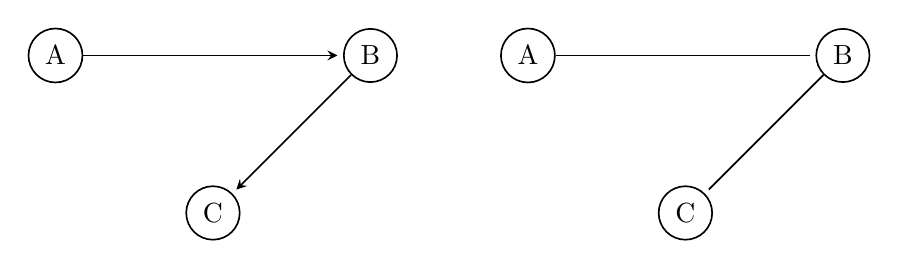
\begin{tikzpicture}[
            > = stealth, % arrow head style
            shorten > = 2pt, % don't touch arrow head to node
            auto,
            node distance = 3cm, % distance between nodes
            semithick % line style
        ]
\node[shape=circle,draw=black] (A) at (0,0) {A};
\node[shape=circle,draw=black] (B) at (4,0) {B};
\node[shape=circle,draw=black] (C) at (2,-2) {C};

 \path [->] (A) edge node[left] {} (B);
 \path [->] (B) edge node[left] {} (C);


\node[shape=circle,draw=black] (A) at (6,0) {A};
\node[shape=circle,draw=black] (B) at (10,0) {B};
\node[shape=circle,draw=black] (C) at (8,-2) {C};

\path [-] (A) edge node[left] {} (B);
\path [-] (B) edge node[left] {} (C);
\end{tikzpicture}
\caption{Graphs corresponding to $V = \{A,B,C\}$, $E = \{(A,B), (B,C)\}$ (left) and , $E = \{(A,B), (B,A), (B,C), (C,B)\}$ (right). } \label{fig:M1}
\end{figure}

 Often times we are interested in how different nodes in a particular graph are or are not connected to one another. In this spirit we define paths.
 
\begin{definition}
A $\mathbf{path}$ $p$ between nodes $v_1, v_n$ is a sequence $v_1, v_2, ..., v_n$  of distinct nodes such that a distinct edge always exists between $v_i$ and $v_{i+1}$. When $v_i \rightarrow v_{i+1} \in E$ for all $i \in \{1,2,...,n \}$, we say $p$ is a $\mathbf{directed \ path}$.
\end{definition}




For a directed graph $G$ and a particular node $v \in V$, we define several sets of related nodes. The \textbf{parents} of $v$, $PA_v$ are the nodes with a directed edge ending at $v$, $\{i \in V | i \rightarrow v \}$ and similarly the \textbf{children} of $v$ are those nodes which $v$ has a directed edge to, $\{i \in V | v \rightarrow i \}$. Notice that in a directed graph, a node cannot be both a child and a parent of any other node. Extending these definitions, we define the \textbf{ancestors} of $v$, $AN_v$, as all the nodes from which a directed path to $v$ exists,  $\{i \in V | i \rightarrow ... \rightarrow v \}$. Likewise we define \textbf{descendants} $DE_v$ of $v$ as the nodes for which a directed path from $v$ exists,   $\{i \in V | v \rightarrow ... \rightarrow i \}$ [ref Peters chp 6.1]. With these in place, we progress to the next definition.

\begin{definition}
A directed graph $G = (V,E)$ is said to be an \emph{\textbf{directed acyclic graph}} (DAG) if for all nodes $v \in V$, $DE_v \cap AN_v = \emptyset$. That is, a directed graph is a DAG when the existence of directed path from $v_1$ to $v_2$ implies that there is not a directed path from $v_2$ to $v_1$.
\end{definition}

\begin{figure}
\centering
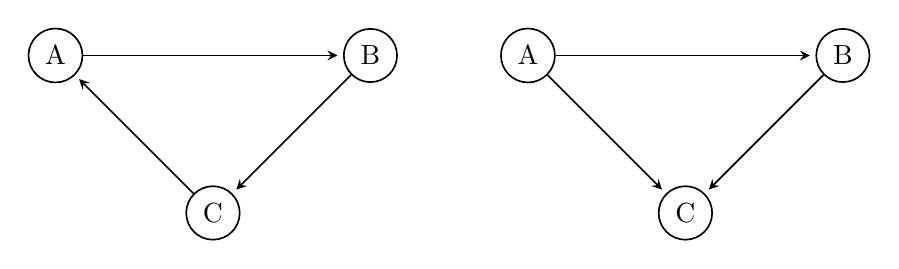
\begin{tikzpicture}[
            > = stealth, % arrow head style
            shorten > = 2pt, % don't touch arrow head to node
            auto,
            node distance = 3cm, % distance between nodes
            semithick % line style
        ]
\node[shape=circle,draw=black] (A) at (0,0) {A};
\node[shape=circle,draw=black] (B) at (4,0) {B};
\node[shape=circle,draw=black] (C) at (2,-2) {C};

 \path [->] (A) edge node[left] {} (B);
 \path [->] (B) edge node[left] {} (C);
  \path [->] (C) edge node[left] {} (A);


\node[shape=circle,draw=black] (A) at (6,0) {A};
\node[shape=circle,draw=black] (B) at (10,0) {B};
\node[shape=circle,draw=black] (C) at (8,-2) {C};

\path [->] (A) edge node[left] {} (B);
\path [->] (B) edge node[left] {} (C);
\path [->] (A) edge node[left] {} (C);
\end{tikzpicture}

\caption{Cyclic (left) and acyclic (right) graphs on the nodes $A,B,C$} \label{fig:M1}
\end{figure}

Now that we have defined DAGs, we can advance to one of our fundamental tools for analyzing them, Pearl's d-separation.

\subsection{D-Separation}
The graphical structure that every SCM entails allows us to reason about the causal and statistical relationships using the properties of directed graphs. One of the essential such tools is d-separation. To develop the intuition, consider the very basic DAG $A \rightarrow B \rightarrow C$. There is exactly one directed path from $A$ to $C$, and the path passes through $B$. So to get to $C$ from $A$ you need to pass through $B$. In this way, we say that $B$ blocks the directed path from $A$ to $C$. We extend this notion [ref Pearl 2008], [ref Peters 2017].

\begin{definition}
Given a directed graph $G$, a path from node $v_1$ to node $v_n$ is said to be \textbf{\emph{blocked}} by a set $S$ (with $S \cap \{v_1, v_n\} = \emptyset$) if:
\begin{enumerate}
\item $v_j \in S$ and $p$ contains a $\mathbf{chain}$: $v_{j-1} \rightarrow v_j \rightarrow v_{j+1}$ or $v_{j-1} \leftarrow v_j \leftarrow v_{j+1}$, or

\item $v_j \in S$ and $p$ contains a \textbf{\emph{fork}}: $v_{j-1} \leftarrow v_j \rightarrow v_{j+1}$, or

\item $v_j \notin S$ and $DE_{v_j} \cap S = \emptyset$ and $p$ contains a \textbf{\emph{collider}}: $v_{j-1} \rightarrow v_j \leftarrow v_{j+1}$. As we will see, colliders play an especially important role in the analysis of causal DAGs.
\end{enumerate}
\end{definition}

\begin{example}
Consider a path $A \rightarrow B \rightarrow C \leftarrow D \rightarrow E$ between nodes $A$ and $E$. There are many sets that block this path. For one, there is a collider on the path. This means that any set which does not include $C$ or any elements of $DE_C$ would successfully block the path. However, we could also pick $S = \{B\}$, $S= \{D\}$, or $S = \{B,D\}$ as blocking sets since the path contains a chain at $B$ and a  fork at $D$. Importantly, if we have either of these nodes in our blocking set, we could include $C$ as well because the first blocking condition would be satisfied, even though the second would not. In fact, the only $S \subseteq \{B,C,D\}$ that would not block the path is $S = \{C\}$.
\end{example}

With blocking defined, we address d-separation. 

\begin{definition}
For a DAG $G$, two sets of nodes $A,B \in G$ are said to be  \textbf{\emph{d-separated}} by a set $S$ if all paths between $A$ and $B$ are blocked by $S$. We denote d-separation by the symbol $\perp \!\!\!\perp_G$, with the statement "$A$ is d-separated from $B$ by $S$" expressed as $A \dsep_G B | S$. 
\end{definition}

\begin{remark}
If $A \dsep_G B | S$ then $B \dsep_G A | S$
\end{remark}
\begin{example}
Consider the DAG $G$ below.

    $$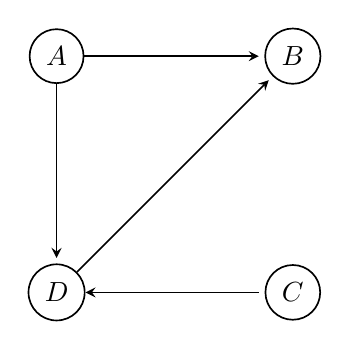
\begin{tikzpicture}[
            > = stealth, % arrow head style
            shorten > = 2pt, % don't touch arrow head to node
            auto,
            node distance = 3cm, % distance between nodes
            semithick % line style
        ]
        

        \tikzstyle{every state}=[
            draw = black,
            thick,
            fill = white,
            minimum size = 4mm
        ]

        \node[shape=circle,draw=black] (A) {$A$};
        \node[shape=circle,draw=black] (B) [right of=A] {$B$};
        \node[shape=circle,draw=black] (C) [below of=B] {$C$};
        \node[shape=circle,draw=black] (D) [left of=C] {$D$};

        \path[->] (A) edge node {} (B);
	    \path[->] (A) edge node {} (D);
	    \path[->] (D) edge node {} (B);
	    \path[<-] (D) edge node {} (C);
    \end{tikzpicture}$$
\end{example}

Which nodes can be d-separated, and by which blocking sets? Nodes which are connected by an edge cannot be d-separated. To see why, take $A$ and $B$. Although some paths between $A$ and $B$ can be blocked, the path $A \rightarrow B$ contains no nodes other than $A$ and $B$ and therefore cannot be blocked. Since there is no set that can block the path, $A$ and $B$ are not able to be d-separated. So consider $A$ and $C$, two nodes which are not connected by an edge. There are two paths between $A$ and $C$, $A \rightarrow B \leftarrow D \leftarrow C$ and $A \rightarrow D \leftarrow C$. Both of these paths include a collider. Of the four possible blocking sets, $\emptyset, \{B\}, \{D\}, \{B,D\}$, all but $\emptyset$ include a collider node for paths that are not blocked by other means. Then $A \dsep_G C | \emptyset$ and no other sets will work. What about $B$ and $C$? Again there are two paths: $B \leftarrow D \leftarrow C$ and $B \leftarrow A \rightarrow D \leftarrow C$. The second path contains a collider, and therefore is blocked by $\emptyset$, but the first path cannot be. To block $B \leftarrow D \leftarrow C$ we must have $D$ in our blocking set. So, $B \dsep_G C | D$, but we can also include $A$ since doing so will not unblock a path with a collider. Then $B \dsep_G C | D,A$.


\begin{theorem}
Two nodes in a DAG $G$ can be d-separated if and only if there is not an edge between the two nodes. 
\end{theorem}

\subsection{Structural Causal Models}
A huge array of questions in the natural and social sciences revolve around understanding the way that one set of factors (e.g. genes, medicines, social policies) influence others (e.g. disease risk, mortality, childhood poverty rates). In these cases, the language and  of classical statistics is often inadequate. The tools of hypothesis testing, (linear) regression, interval estimation, ect. can tell us much about relationships in the data, but except in the highly constrained setting of randomized controlled trials, very little about cause and effect. These limitations are not just theoretical. Many longstanding controversies and debates within the sciences come down to disagreements over which factors associated with a particular outcome are causing the outcome. 

A paradigmatic example of such a controversy is over the relationship between cigarette smoking and lung cancer. Today, it is uncontroversial that smoking cigarettes (especially habitually over a long period of time) increases a person's risk of contracting lung cancer. This is a causal relationship, and we might express our belief in this relationship as a \textbf{\emph{causal model}} in which a person's risk of contracting lung cancer is a \emph{function} of a person's smoking habits (for simplicity, we  pretend that smoking is the only such causal factor).

So, let $L$ be a random variable denoting whether or not a person contracts lung cancer and $S$ be a random variable denoting smoking. Under our causal model in which smoking is the only structural cause of lung cancer, we express $L$ as a function of $S$:

$$L :=f(S, N_L),$$
$$S := N_S.$$ 

Here, the use of $:=$ denotes an assignment rather that an algebraic relationship [ref Peters] and $N_L$ is a noise term capturing random effects on lung cancer risk, and $N_S$ a noise variable for cigarette smoking. Together, these two assignments are a  structural causal model.  Now that we have an SCM, we can express the structure as a DAG. Since $L$ is assigned as a function of smoking but $S$ is not caused by any factors in our model, we would express our model as a directed edge going from $S$ to L:



$$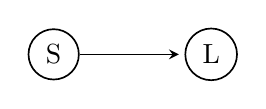
\begin{tikzpicture}[
            > = stealth, % arrow head style
            shorten > = 2pt, % don't touch arrow head to node
            auto,
            node distance = 3cm, % distance between nodes
            semithick % line style
        ]
\node[shape=circle,draw=black] (S) at (8,0) {S};
\node[shape=circle,draw=black] (L) at (10,0) {L};


 \path [->] (S) edge node[left] {} (L);



\end{tikzpicture}$$

However, historically, this causal structure was not the only one suggested to explain the association between lung cancer and smoking. One particularly illustrious detractor of this theory was British statistician R. A. Fisher, a foundational figure in modern statistics (and a heavy smoker) [ref Fisher]. In Fisher's view, there was no causal effect of smoking on lung cancer, rather, an underlying genetic factor was responsible for both a predisposition to smoking and a higher risk of developing lung cancer. So Fisher's causal model would have looked like:
$$L :=f(G, N_L),$$
$$S := f(G, N_S),$$
$$G := N_G.$$ 
Where $G$ is the genetic factor. As before, the structure of this model can be expressed as a graph:

$$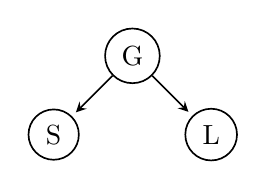
\begin{tikzpicture}[
            > = stealth, % arrow head style
            shorten > = 2pt, % don't touch arrow head to node
            auto,
            node distance = 3cm, % distance between nodes
            semithick % line style
        ]
\node[shape=circle,draw=black] (G) at (9,1) {G};
\node[shape=circle,draw=black] (S) at (8,0) {S};
\node[shape=circle,draw=black] (L) at (10,0) {L};

 \path [->] (G) edge node[left] {} (L);
 \path [->] (G) edge node[left] {} (S);
\end{tikzpicture}$$


In this way, every SCM entails a directed graph. Although it is entirely possible for an SCM to entail a graph that has cycles, we focus our attention on the case where the graph entailed is a DAG. Importantly, these two (graphical) models imply different observational joint distributions. Without having specified the functions, little can be said about the joint distribution entailed by the model, however, one important property is built in to every SCM.

\begin{definition}[Markov property]
In any SCM $C$ with entailed graph $G$, if $A \dsep_G B | S \implies A \dsep B | S$ for all disjoint sets of nodes $A,B,S$. That is, every d-separation in the graph corresponds to a conditional independence in the joint distribution. This fact is implied by the definition of SCMs and is called the \emph{\textbf{Markov Property}}.
\end{definition}

[This seems important enough to reproduce a proof but I will have to spend a little more time than I have tonight]

This result is a powerful tool that allows us to test how well differing causal models comport with the observational data.  Returning to Fisher's suggestion that an underlying genetic cause was responsible for the association of smoking with lung cancer, consider that by the Markov property $S \dsep L | G$. Let's assume we have a population of identical twins, some of whom were smoking discordant. Since we know that identical twins are genetically identical  we could assess whether or not smoking and lung cancer are independent within twin pairs. If not, then something must be wrong with the model. 



\end{document}
 